\documentclass[tikz,border=4pt]{standalone}
\usepackage{amsmath}
\definecolor{curveblue}{HTML}{245C86}
\begin{document}
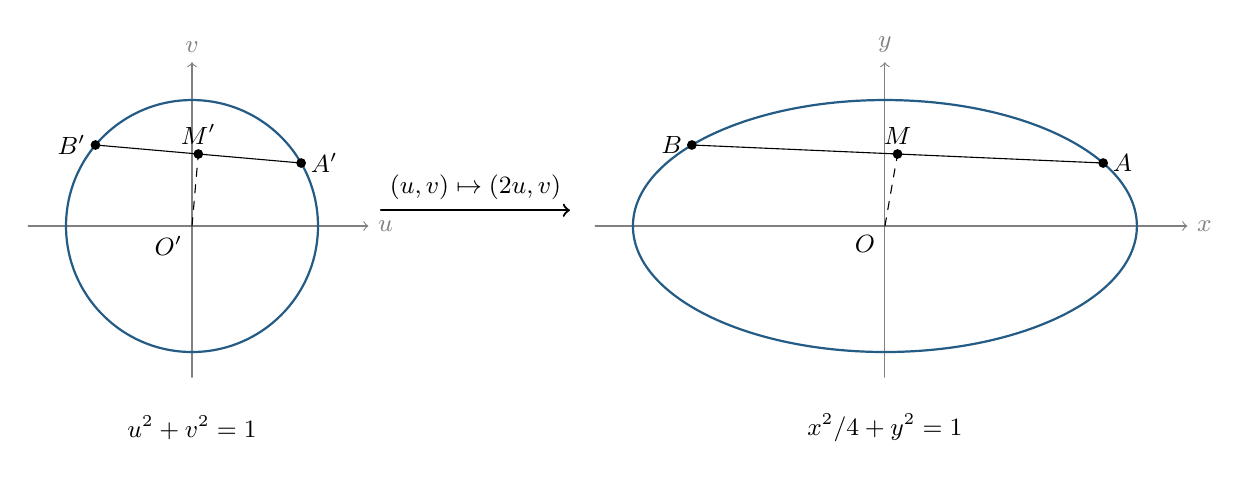
\begin{tikzpicture}[line cap=round,font=\small]
\begin{scope}[scale=1.6]
\draw[gray,->](-1.3,0)--(1.4,0)node[right]{$u$};
\draw[gray,->](0,-1.2)--(0,1.3)node[above]{$v$};
\draw[curveblue,thick](0,0)circle(1);
\coordinate(A)at(.866,.5);\coordinate(B)at(-.766,.643);\coordinate(M)at(.05,.5715);
\draw(A)--(B);\draw[dashed](0,0)--(M);
\fill(A)circle(1.1pt)node[right]{$A'$};\fill(B)circle(1.1pt)node[left]{$B'$};
\fill(M)circle(1.1pt)node[above]{$M'$};\node[below left]at(0,0){$O'$};
\node at(0,-1.6){$u^2+v^2=1$};
\end{scope}
\draw[->,thick](2.4,.2)--(4.8,.2)node[midway,above]{$(u,v)\mapsto(2u,v)$};
\begin{scope}[shift={(8.8,0)},scale=1.6]
\draw[gray,->](-2.3,0)--(2.4,0)node[right]{$x$};
\draw[gray,->](0,-1.2)--(0,1.3)node[above]{$y$};
\draw[curveblue,thick](0,0)ellipse[x radius=2,y radius=1];
\coordinate(A)at(1.732,.5);\coordinate(B)at(-1.532,.643);\coordinate(M)at(.1,.5715);
\draw(A)--(B);\draw[dashed](0,0)--(M);
\fill(A)circle(1.1pt)node[right]{$A$};\fill(B)circle(1.1pt)node[left]{$B$};
\fill(M)circle(1.1pt)node[above]{$M$};\node[below left]at(0,0){$O$};
\node at(0,-1.6){$x^2/4+y^2=1$};
\end{scope}
\end{tikzpicture}
\end{document}
